%  Architecture.tex
%  Document created by seblovett on seblovett-Ubuntu
%  Date created: Thu 17 Apr 2014 14:55:41 BST
%  <+Last Edited: Sun 11 May 2014 10:13:31 BST by seblovett on seblovett-Ubuntu +>


\chapter{Architecture}

\review{Architecture}

%Design of the datapath architecture.

%Refer to the research done and how this influenced the design

The architecture for the processor was initially base upon a MIPS style datapath.
Support was then added to allow the ARM Thumb instruction set (see Chapter~\ref{ch:is}) to be executed on the datapath.
Extra aspects of the datapath were then added based on the research done. 
The full datapath diagram is seen in Figure~\ref{fig:architecture}.

A dedicated Link Register is used to improve the speed when calling leaf functions.
The original design also included a dedicated Stack Pointer, however this was later removed during the project due to the need for specialist instructions.
The convention of using Register 7 as the Stack Pointer was instead used. 
Both of these aspects were added from the recommendations from the research report on subroutines.

The processor supports four flags: carry, overflow, negative and zero. 
It is a two operand register-register design.
There are eight general purpose registers with no dummy register. 

The datapath was also modified during the project to allow for interrupt support.
These changes included an input to the Program Counter to jump to a specific location, reading and writing of the status register from and to the system bus, and input of the Program Counter directly from the system bus. 


\begin{figure}
%%\missingfigure{Architecture diagram}
%\hspace*{-1in}
\vspace*{-1in}
\setlength{\abovecaptionskip}{0pt}
\setlength{\belowcaptionskip}{0pt}
\makebox[\linewidth]{
\centerline{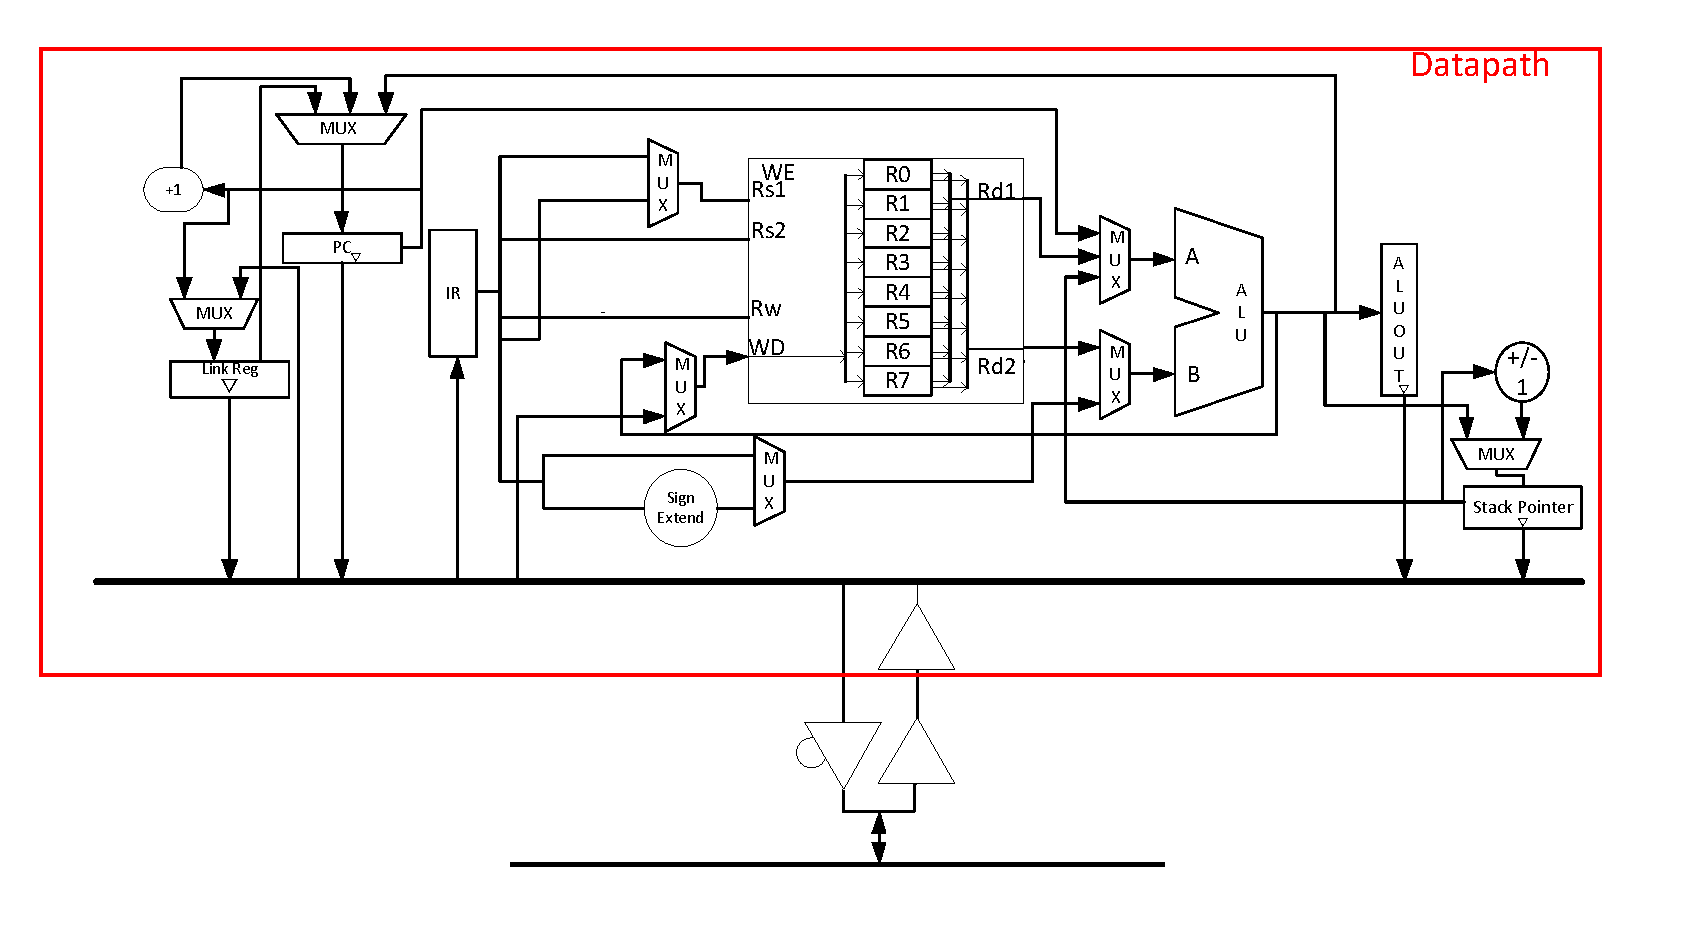
\includegraphics[angle=270,scale=0.9]{../../Design/RandD/idea1.pdf}}
}
\caption{The Architecture diagram of the processor.}
\label{fig:architecture}
\end{figure}
\todo[inline, color=green]{MW: would this need re-angling so bottom edge on outside edge of book?}

